\documentclass{standalone}
\usepackage{tikz}
\begin{document}
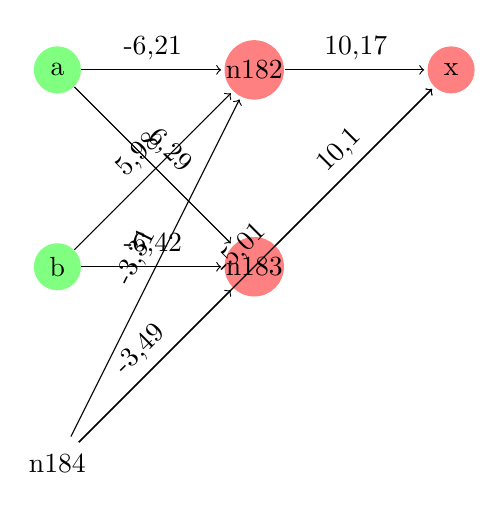
\begin{tikzpicture}[shorten >=1pt,->,draw=black!,node distance=2.5cm]
\tikzstyle{neuron}=[circle,fill=black!25,minimum size=17pt,inner sep=0pt]
\tikzstyle{constant}=[neuron, fill=white!50];
\tikzstyle{identity}=[neuron, fill=green!50];
\tikzstyle{sigmoid}=[neuron, fill=red!50];
\node [identity] (a) {a};
\node [identity,below of=a] (b) {b};
\node [constant,below of=b] (n184) {n184};
\node [sigmoid,right of=a] (n182) {n182};
\node [sigmoid,below of=n182] (n183) {n183};
\node [sigmoid,right of=n182] (x) {x};
\path[every node/.style={sloped,anchor=south,auto=false}]
(a) edge node {-6,21} (n182)
(a) edge node {6,29} (n183)
(b) edge node {5,98} (n182)
(b) edge node {-6,42} (n183)
(n184) edge node {-3,49} (n183)
(n184) edge node {-3,31} (n182)
(n184) edge node {-5,01} (x)
(n182) edge node {10,17} (x)
(n183) edge node {10,1} (x)
;\end{tikzpicture}
\end{document}